%==============================================================================
% More Code, Slower Tangle — AI adoption across twenty MOSIP core services
%
% TO USE IN OVERLEAF
%   1. New Project -> Upload Project -> zip this whole `paper/` folder
%   2. Main document: main.tex   Compiler: pdfLaTeX
%   3. Compiles with no uploads; every package ships with Overleaf
%
% Styled to match the web report: single measured column, sage palette, tinted
% result boxes. All presentation lives in preamble.tex; this file is content.
%
% TO SUBMIT TO AN ACM VENUE (MSR etc.) the original acmart version is kept at
% main-acmart.tex.bak — the prose is identical, so the section bodies copy
% across unchanged.
%==============================================================================
\documentclass[11pt,a4paper]{article}
%==============================================================================
% preamble.tex — visual identity matching the web report
%
% Palette, type and box styles are lifted from the HTML version so the PDF and
% the artifact read as the same document. Everything here is presentation; no
% content lives in this file.
%==============================================================================

%------------------------------------------------------------------------------
% PALETTE  (same hex values as the web report's CSS custom properties)
%------------------------------------------------------------------------------
\usepackage[table,dvipsnames]{xcolor}
\definecolor{paper}{HTML}{EEF0EA}   % page ground (sage-grey)
\definecolor{raised}{HTML}{F6F7F3}  % box fill, one step lighter
\definecolor{ink}{HTML}{1B211C}     % body text, green-black
\definecolor{muted}{HTML}{5F6A62}   % captions, secondary
\definecolor{rule}{HTML}{CDD3C9}    % hairlines
\definecolor{rulesoft}{HTML}{DFE3DA}
\definecolor{pine}{HTML}{2C5C4C}    % structural accent
\definecolor{pinesoft}{HTML}{DCE6DF}
\definecolor{rust}{HTML}{A2432B}    % semantic: worse / caution
\definecolor{slate}{HTML}{40628C}   % semantic: better / down
\definecolor{amber}{HTML}{8A6A1F}   % findings

\color{ink}
% The web version sits on a tinted ground. On paper that costs ink and hurts
% print legibility, so the page stays white and the tint is reserved for boxes.
% Uncomment for an on-screen version that matches the artifact exactly:
% \pagecolor{paper}

%------------------------------------------------------------------------------
% TYPE
% The web report uses Spectral / Public Sans / IBM Plex Mono. Those are Google
% fonts; the Adobe Source trio below is the closest pairing that ships with
% Overleaf and compiles under pdfLaTeX with no uploads. Source Serif stands in
% for Spectral, Source Sans for Public Sans, Source Code Pro for Plex Mono.
%
% FOR THE EXACT WEB FONTS: switch the compiler to XeLaTeX or LuaLaTeX, upload
% the .ttf files, and replace this block with:
%   \usepackage{fontspec}
%   \setmainfont{Spectral}[Numbers=OldStyle]
%   \setsansfont{Public Sans}
%   \setmonofont{IBM Plex Mono}[Scale=0.88]
%   \renewcommand{\familydefault}{\sfdefault}
%------------------------------------------------------------------------------
\usepackage[T1]{fontenc}
\usepackage{sourceserifpro}                 % \rmfamily — headings
\usepackage[scale=0.96]{sourcesanspro}      % \sffamily — body
\usepackage[scale=0.86]{sourcecodepro}      % \ttfamily — data
\renewcommand{\familydefault}{\sfdefault}   % body is sans, as on the web
\usepackage{microtype}
% letterspace (microtype bundle) handles macros inside the argument;
% soul's \so does not and fails with 'Reconstruction failed'.
\usepackage{letterspace}

%------------------------------------------------------------------------------
% PAGE — single measured column, like the web report
%------------------------------------------------------------------------------
\usepackage[a4paper,margin=30mm,top=26mm,bottom=28mm]{geometry}
\linespread{1.10}
\setlength{\parskip}{0.62em}
\setlength{\parindent}{0pt}                  % web-style blocks, no indents
\usepackage{ragged2e}
\RaggedRight                                 % unjustified, as on screen

%------------------------------------------------------------------------------
% HEADINGS
%------------------------------------------------------------------------------
\usepackage{titlesec}
\titleformat{\section}
  {\rmfamily\bfseries\LARGE\color{ink}}{}{0pt}{}
\titlespacing*{\section}{0pt}{2.1em}{0.55em}
\titleformat{\subsection}
  {\rmfamily\bfseries\large\color{ink}}{\thesubsection\quad}{0pt}{}
\titlespacing*{\subsection}{0pt}{1.5em}{0.4em}
\titleformat{\paragraph}[runin]
  {\sffamily\bfseries\color{ink}}{}{0pt}{}[.]
\titlespacing*{\paragraph}{0pt}{0.9em}{0.5em}

% "eyebrow" — the small uppercase mono label above a section on the web
\newcommand{\eyebrow}[1]{%
  \par\vspace{0.4em}%
  {\ttfamily\footnotesize\color{pine}\textls[120]{\MakeUppercase{#1}}}\par\vspace{-0.5em}}

% section with an eyebrow above it
\newcommand{\esection}[2]{\eyebrow{#1}\section{#2}}

%------------------------------------------------------------------------------
% BOXES
%------------------------------------------------------------------------------
\usepackage[most]{tcolorbox}
\tcbset{
  boxrule=0pt, arc=0.6mm, left=5mm, right=5mm, top=3.2mm, bottom=3.2mm,
  boxsep=0mm, colback=raised, enhanced, breakable
}
% research-question block — pine rule on the left
\newtcolorbox{rqbox}{borderline west={2.4pt}{0pt}{pine}}
% finding — amber rule across the top, the headline result of a section
\newtcolorbox{findingbox}[1]{%
  borderline north={2.4pt}{0pt}{amber},
  title={\ttfamily\footnotesize\color{amber}\textls[120]{\MakeUppercase{#1}}},
  coltitle=amber, fonttitle=\ttfamily, attach title to upper=\par\vspace{1.5mm},
  colbacktitle=raised, titlerule=0pt, boxed title style={empty}}
% caution — rust rule on the left, for competing explanations
\newtcolorbox{cautionbox}[1]{%
  borderline west={2.4pt}{0pt}{rust},
  title={\sffamily\bfseries\color{rust}#1},
  coltitle=rust, attach title to upper=\par\vspace{1.5mm},
  colbacktitle=raised, titlerule=0pt, boxed title style={empty}}
% constructive — pine rule on the left
\newtcolorbox{goodbox}[1]{%
  borderline west={2.4pt}{0pt}{pine},
  title={\sffamily\bfseries\color{pine}#1},
  coltitle=pine, attach title to upper=\par\vspace{1.5mm},
  colbacktitle=raised, titlerule=0pt, boxed title style={empty}}

%------------------------------------------------------------------------------
% TABLES — booktabs rules, mono figures, tinted rows for significant results
%------------------------------------------------------------------------------
\usepackage{booktabs}
\usepackage{tabularx}
\usepackage{siunitx}
\sisetup{group-separator={,},detect-all=true}
\renewcommand{\arraystretch}{1.22}
\setlength{\aboverulesep}{0pt}\setlength{\belowrulesep}{0pt}
\arrayrulecolor{rule}

% column type for numeric cells: mono, right-aligned, tabular figures
\newcolumntype{N}{>{\ttfamily}r}
% tint a row whose result reached significance
\newcommand{\sigrow}{\rowcolor{pinesoft}}
% inline emphasis inside tables
\newcommand{\sig}[1]{\textbf{#1}}
\newcommand{\up}[1]{\textcolor{rust}{#1}}
\newcommand{\dn}[1]{\textcolor{slate}{#1}}
\newcommand{\nil}[1]{\textcolor{muted}{#1}}

% table captions above, small, muted
\usepackage[font={small,color=muted},labelfont={bf,color=ink},
            justification=raggedright,singlelinecheck=false,skip=5pt]{caption}

%------------------------------------------------------------------------------
% FIGURES
%------------------------------------------------------------------------------
% `float` gives [H]: tables land exactly where written instead of drifting
% above the heading they belong to, which matches the web report.
\usepackage{float}
\usepackage{graphicx}
\graphicspath{{figures/}}

%------------------------------------------------------------------------------
% LISTS — web-like spacing
%------------------------------------------------------------------------------
\usepackage{enumitem}
\setlist[itemize]{leftmargin=1.2em,itemsep=0.45em,topsep=0.4em}
\setlist[enumerate]{leftmargin=1.5em,itemsep=0.55em,topsep=0.4em}
\setlist[description]{leftmargin=0pt,itemsep=0.5em,topsep=0.4em,
                      font=\ttfamily\footnotesize\color{pine}}

%------------------------------------------------------------------------------
% MISC
%------------------------------------------------------------------------------
\usepackage{amsmath}
\usepackage[hidelinks]{hyperref}
\hypersetup{colorlinks=true,linkcolor=pine,citecolor=pine,urlcolor=pine}
\newcommand{\evt}{\tau}
% \colorbox is unbreakable and overflows the measure on long identifiers;
% \allowbreak lets a line break after an inline code span instead.
\newcommand{\code}[1]{%
  {\ttfamily\small\colorbox{pinesoft}{\hspace{0.15em}#1\hspace{0.15em}}}\allowbreak}
% \codep — for long paths and identifiers. A \colorbox is a single unbreakable
% object, so a long one runs into the margin; this keeps the mono face and
% drops the tint so the line can break normally.
\newcommand{\codep}[1]{{\ttfamily\small #1}}

% running footer, mono and muted, like the web footer
\usepackage{fancyhdr}
\pagestyle{fancy}\fancyhf{}
\renewcommand{\headrulewidth}{0pt}
\fancyfoot[C]{\ttfamily\scriptsize\color{muted}\thepage}

% title block
\newcommand{\reportheader}[4]{%
  {\ttfamily\footnotesize\color{pine}\textls[120]{\MakeUppercase{#1}}}\par\vspace{1.1em}
  {\rmfamily\bfseries\fontsize{26}{29}\selectfont\color{ink}#2}\par\vspace{0.7em}
  {\rmfamily\large\color{ink}#3}\par\vspace{0.9em}
  {\ttfamily\scriptsize\color{muted}#4}\par\vspace{0.5em}
  {\color{rule}\rule{\linewidth}{0.5pt}}\par\vspace{1.2em}}


\begin{document}

\reportheader
  {Working draft \textperiodcentered\ Upanzi \textperiodcentered\ 24 September 2026}
  {More code, slower tangle}
  {AI adoption across twenty MOSIP core services: what changed in code volume,
   code quality and code-review practice, reported in absolute terms.}
  {20 repositories \quad 326 repo-months \quad 6,786 commits \quad
   5,603 pull requests \quad window 2025-01 $\rightarrow$ 2026-08}

%==============================================================================
\esection{1 \textperiodcentered\ Introduction}{Motivation}
\label{sec:intro}

The claim that AI coding assistants trade short-term speed for long-term
maintainability is now widely repeated and has recent empirical support. He
et~al.~\cite{he2026speed} report that Cursor adoption raises velocity while
worsening complexity growth across a large population of open-source projects,
estimating an \emph{average} effect using difference-in-differences against
matched controls.

This work asks a narrower question with a different unit of analysis: what
happens inside \emph{one} organisation? MOSIP is digital public infrastructure
--- the identity platform deployed by several national governments --- so its
code is long-lived, security-sensitive, and maintained by a stable engineering
organisation rather than a churning volunteer pool. If AI assistance degrades
maintainability anywhere, this is a setting where the consequences matter.

MOSIP also proves to be an unusually clean natural setting, for a reason that
emerged only during data collection: the organisation adopted \textbf{two
different classes of AI tool, seven months apart}. An AI code \emph{reviewer}
arrived first, organisation-wide; AI code \emph{writers} followed. These are
distinct interventions with distinct predicted effects, and prior work
generally collapses them.

\begin{rqbox}
\setlength{\parskip}{0.7em}
\textbf{RQ1 --- Volume.}\enspace Did the amount of code, and the rate at which
it is produced, change after AI coding agents were adopted?\par
\textbf{RQ2 --- Quality.}\enspace Did internal code quality --- complexity,
code smells, technical debt --- change after adoption?\par
\textbf{RQ3 --- Review practice.}\enspace Did an AI code-review bot substitute
for human review effort, or add to it?
\end{rqbox}

%==============================================================================
\esection{2 \textperiodcentered\ Methods}{Subjects, data and design}
\label{sec:methods}

\subsection{Repository selection}
\label{sec:selection}

The MOSIP GitHub organisation holds 109 public repositories, 97 of them neither
archived nor forks. Ranking by stars is uninformative here --- the whole
organisation spans 4 to 87 stars --- and promotes artefacts with no analysable
code, such as \code{documentation} (794\,MB of prose) and the empty
\code{mosip} meta-repository.

We instead ranked by \textbf{JVM source volume} obtained from the GitHub
languages API, after excluding by name mocks, test harnesses, deployment and
infrastructure repositories, configuration repositories and documentation. That
left 36 candidate core services, of which we took the \textbf{top 20 by source
volume}, totalling 47.2\,MB of JVM source. Checkout size was rejected as a
criterion because it is inflated by history and binaries: \code{packet-manager}
occupies 188\,MB on disk but holds only 0.51\,MB of Java.

\subsection{Data collection}
\label{sec:collection}

Three independent sources were collected in September 2026 over a window of
2025-01 to 2026-08 (Table~\ref{tab:data}).

\begin{table}[H]
\caption{Data sources and coverage.}
\label{tab:data}
\small
\begin{tabularx}{\linewidth}{@{}lXr@{}}
\toprule
\textbf{Source} & \textbf{Extracted} & \textbf{Volume} \\
\midrule
Git history & commits, lines $\pm$, contributors & {\ttfamily 6,786} commits \\
            &                                    & {\ttfamily 3.19M} lines added \\
\addlinespace[3pt]
GitHub API  & pull requests, reviews, issues     & {\ttfamily 5,603} PRs \\
            &                                    & {\ttfamily 17,090} reviews \\
            &                                    & {\ttfamily 1,222} issues \\
\addlinespace[3pt]
SonarQube 26.8 & ncloc, cognitive complexity, code smells, technical debt,
                 bugs, vulnerabilities, duplication & {\ttfamily 286} snapshots \\
            &                                    & {\ttfamily 285/326} (87\%) \\
\bottomrule
\end{tabularx}
\end{table}

SonarQube reports only on a checked-out working tree, so history was
reconstructed by checking out the last commit of each month and re-analysing
the project in full --- 286 independent analyses on a dedicated Linux host.
Months in which nothing landed on the integration branch have no snapshot,
accounting for nearly all of the 13\% shortfall. Analysis ran on source without
compilation, matching the procedure of~\cite{he2026speed}.

Velocity is counted across \emph{all} branches (\code{git log -{}-all}),
because MOSIP follows gitflow and \code{master} held only 2,025 of 6,786
commits in the window; quality snapshots necessarily follow a single
integration branch. The two halves therefore describe different commit sets ---
``all work performed'' versus ``quality of the shippable tree'' --- and are not
strictly commensurable.

\subsection{Detecting adoption}
\label{sec:detection}

Adoption was not self-reported. Three independent signal families were matched
against every repository: commit-message trailers and identities
(\codep{Co-Authored-By: Claude}, \code{cursoragent}), agent configuration files
committed to the tree (\code{CLAUDE.md}, \code{.cursor/}, \code{AGENTS.md}),
and bot accounts acting on GitHub. Detection yielded \textbf{4,288
AI-attributable actions} (Table~\ref{tab:tools}).

\begin{table}[H]
\caption{Detected AI tools and organisation-wide adoption.}
\label{tab:tools}
\small
\begin{tabularx}{\linewidth}{@{}llrX@{}}
\toprule
\textbf{Tool} & \textbf{Class} & \textbf{Actions} & \textbf{Adoption} \\
\midrule
\sigrow CodeRabbit & reviews code & {\ttfamily 4,141} & \textbf{2025-11} (14/19 repos) \\
Cursor       & writes code & {\ttfamily 64} & 2026-03 -- 2026-08 \\
OpenAI Codex & writes code & {\ttfamily 48} & 2026-04 -- 2026-06 \\
Claude Code  & writes code & {\ttfamily 35} & 2026-06 -- 2026-08 \\
\bottomrule
\end{tabularx}
\end{table}

The gap between a repository's review-bot and coding-agent adoption has median
\textbf{7 months} (range 4--9). RQ1 and RQ2 are therefore evaluated against
\textbf{coding-agent} adoption and RQ3 against \textbf{review-bot} adoption.
Collapsing the two attributes code-generation effects to the arrival of a
commenting tool.

\subsection{Analysis design}
\label{sec:design}

Each repository's timeline is re-indexed to event time,
\begin{equation}
  \evt_{it} = t - a_i ,
  \label{eq:eventtime}
\end{equation}
where $a_i$ is repository $i$'s own adoption month, and the twenty series are
pooled by $\evt$.

\textbf{All measures are reported raw.} No normalisation is applied: no ratio
to a pre-adoption baseline, and no division by code size. Figures use
logarithmic axes where repositories span orders of magnitude (\code{ncloc}
ranges from 7,931 to 355,811), but that is a display choice and leaves the
values untouched.

Every test is a \emph{within-repository} comparison, so each repository serves
as its own control and differences in scale between repositories do not
confound the tests themselves. Scale does dominate the pooled box plots, where
the height of each box is largely between-repository size rather than change
over time; the per-repository view in Figure~\ref{fig:perrepo} is provided for
that reason.

Hypothesis tests are computed at the \textbf{repository level}: each repository
contributes one pre-adoption median and one post-adoption median, giving 16--19
independent pairs compared by Wilcoxon signed-rank. Pooling repository-months
would inflate $n$ to roughly 300 and overstate significance, since months
within a repository are strongly autocorrelated. Pre is $\evt\in[-6,-1]$; post
is $\evt\in[+1,+3]$ for RQ1--2 and $[+1,+6]$ for RQ3. The incomplete current
month is excluded throughout.

%==============================================================================
\esection{3 \textperiodcentered\ Results}{Results}
\label{sec:results}

\subsection{Code volume}
\label{sec:volume}

\begin{table}[H]
\caption{Code volume, raw. Repository-level paired medians, Wilcoxon
signed-rank. Tinted rows reached significance.}
\label{tab:volume}
\small
\begin{tabular}{@{}lNNNNNN@{}}
\toprule
\textbf{Measure (raw)} & \textbf{pre} & \textbf{post} & \textbf{ratio} &
\textbf{p} & \textbf{n} & \textbf{up} \\
\midrule
\sigrow Code size (ncloc) & 45,362 & 50,531 & \up{1.11} & \sig{<.0001} & 16 & \sig{16/16} \\
\sigrow Lines removed / mo & 403 & 501 & \up{1.24} & \sig{.007} & 17 & \sig{14/17} \\
Lines added / mo & 1,583 & 3,098 & \up{1.96} & .145 & 17 & 10/17 \\
Lines added / commit & 243.8 & 435.7 & \up{1.79} & .244 & 17 & 9/17 \\
Commits / month & 11.0 & 12.0 & 1.09 & .287 & 17 & 11/17 \\
Contributors / month & 4.5 & 3.5 & \dn{0.78} & .726 & 17 & 5/17 \\
\bottomrule
\end{tabular}
\end{table}

\begin{findingbox}{Finding 1}
Code volume grew unanimously and significantly: every one of the 16
repositories with quality data was larger after adoption, a median increase of
11\% within three months. Deletion activity also rose ($+24\%$, $p=.007$) in 14
of 17 repositories.
\end{findingbox}

Commit \emph{count} did not change ($p=.287$). Commit \emph{size} nearly
doubled in the median (244 $\to$ 436 lines added per commit) but is not
significant and splits 9/17 --- the median moved because a minority of
repositories changed a great deal, not because most did. That measure is also a
monthly mean ($\text{lines} \div \text{commits}$) rather than a distribution
over commits, so a single bulk import dominates its month; \code{nfiq} 2025-09
comprises 2 commits and 36,810 lines. It should be read as indicative only.

Contributors fell 4.5 $\to$ 3.5, far from significance, and in the same
direction as an organisation-wide slowdown discussed in
Section~\ref{sec:threats}.

%==============================================================================
\subsection{Code quality}
\label{sec:quality}

\begin{table}[H]
\caption{Code quality, raw totals.}
\label{tab:quality}
\small
\begin{tabular}{@{}lNNNNNN@{}}
\toprule
\textbf{Measure (raw)} & \textbf{pre} & \textbf{post} & \textbf{ratio} &
\textbf{p} & \textbf{n} & \textbf{up} \\
\midrule
\sigrow Cognitive complexity & 2,703 & 2,762 & \up{1.02} & \sig{.005} & 16 & \sig{14/16} \\
\sigrow Code smells & 790.5 & 827.5 & \up{1.05} & \sig{.011} & 16 & \sig{13/16} \\
\sigrow Duplication (\%) & 9.00 & 8.70 & \dn{0.97} & \sig{.024} & 16 & 3/16 \\
Vulnerabilities & 8.5 & 9.5 & \up{1.12} & .093 & 16 & 5/16 \\
Bugs & 14.0 & 14.0 & 1.00 & .063 & 16 & 6/16 \\
Technical debt (min) & 5,554 & 5,617 & 1.01 & .496 & 16 & 9/16 \\
\bottomrule
\end{tabular}
\end{table}

\begin{findingbox}{Finding 2}
Absolute complexity and code smells rose significantly: complexity in 14 of 16
repositories ($+2\%$, $p=.005$) and smells in 13 of 16 ($+5\%$, $p=.011$).
Technical debt, bugs and vulnerabilities did not move. Duplication \emph{fell}
($-3\%$, $p=.024$) in 13 of 16 repositories.
\end{findingbox}

The increases are consistent in direction but small in magnitude. Read
alongside Finding~1, the same repositories over the same interval added
\textbf{11\% more code} while complexity rose \textbf{2\%} and smells
\textbf{5\%}: the measured quality burden grew, and grew more slowly than the
codebase producing it.

\begin{cautionbox}{What absolute counts can and cannot settle}
A reviewer will ask whether these increases reflect degrading code or simply
more of it. Absolute counts alone cannot separate the two: any codebase that
grows accumulates more complexity points and more smells even when every new
line is written to the same standard as the old. We report absolute values
throughout, so the question is raised here rather than answered.

The relevant evidence available is the juxtaposition above --- 11\% more code
against a 2\% rise in complexity. A size-conditioned analysis, or a model
treating \code{ncloc} as a covariate, would settle it directly and is the
obvious next step.
\end{cautionbox}

\begin{figure}[htbp]
  \centering
  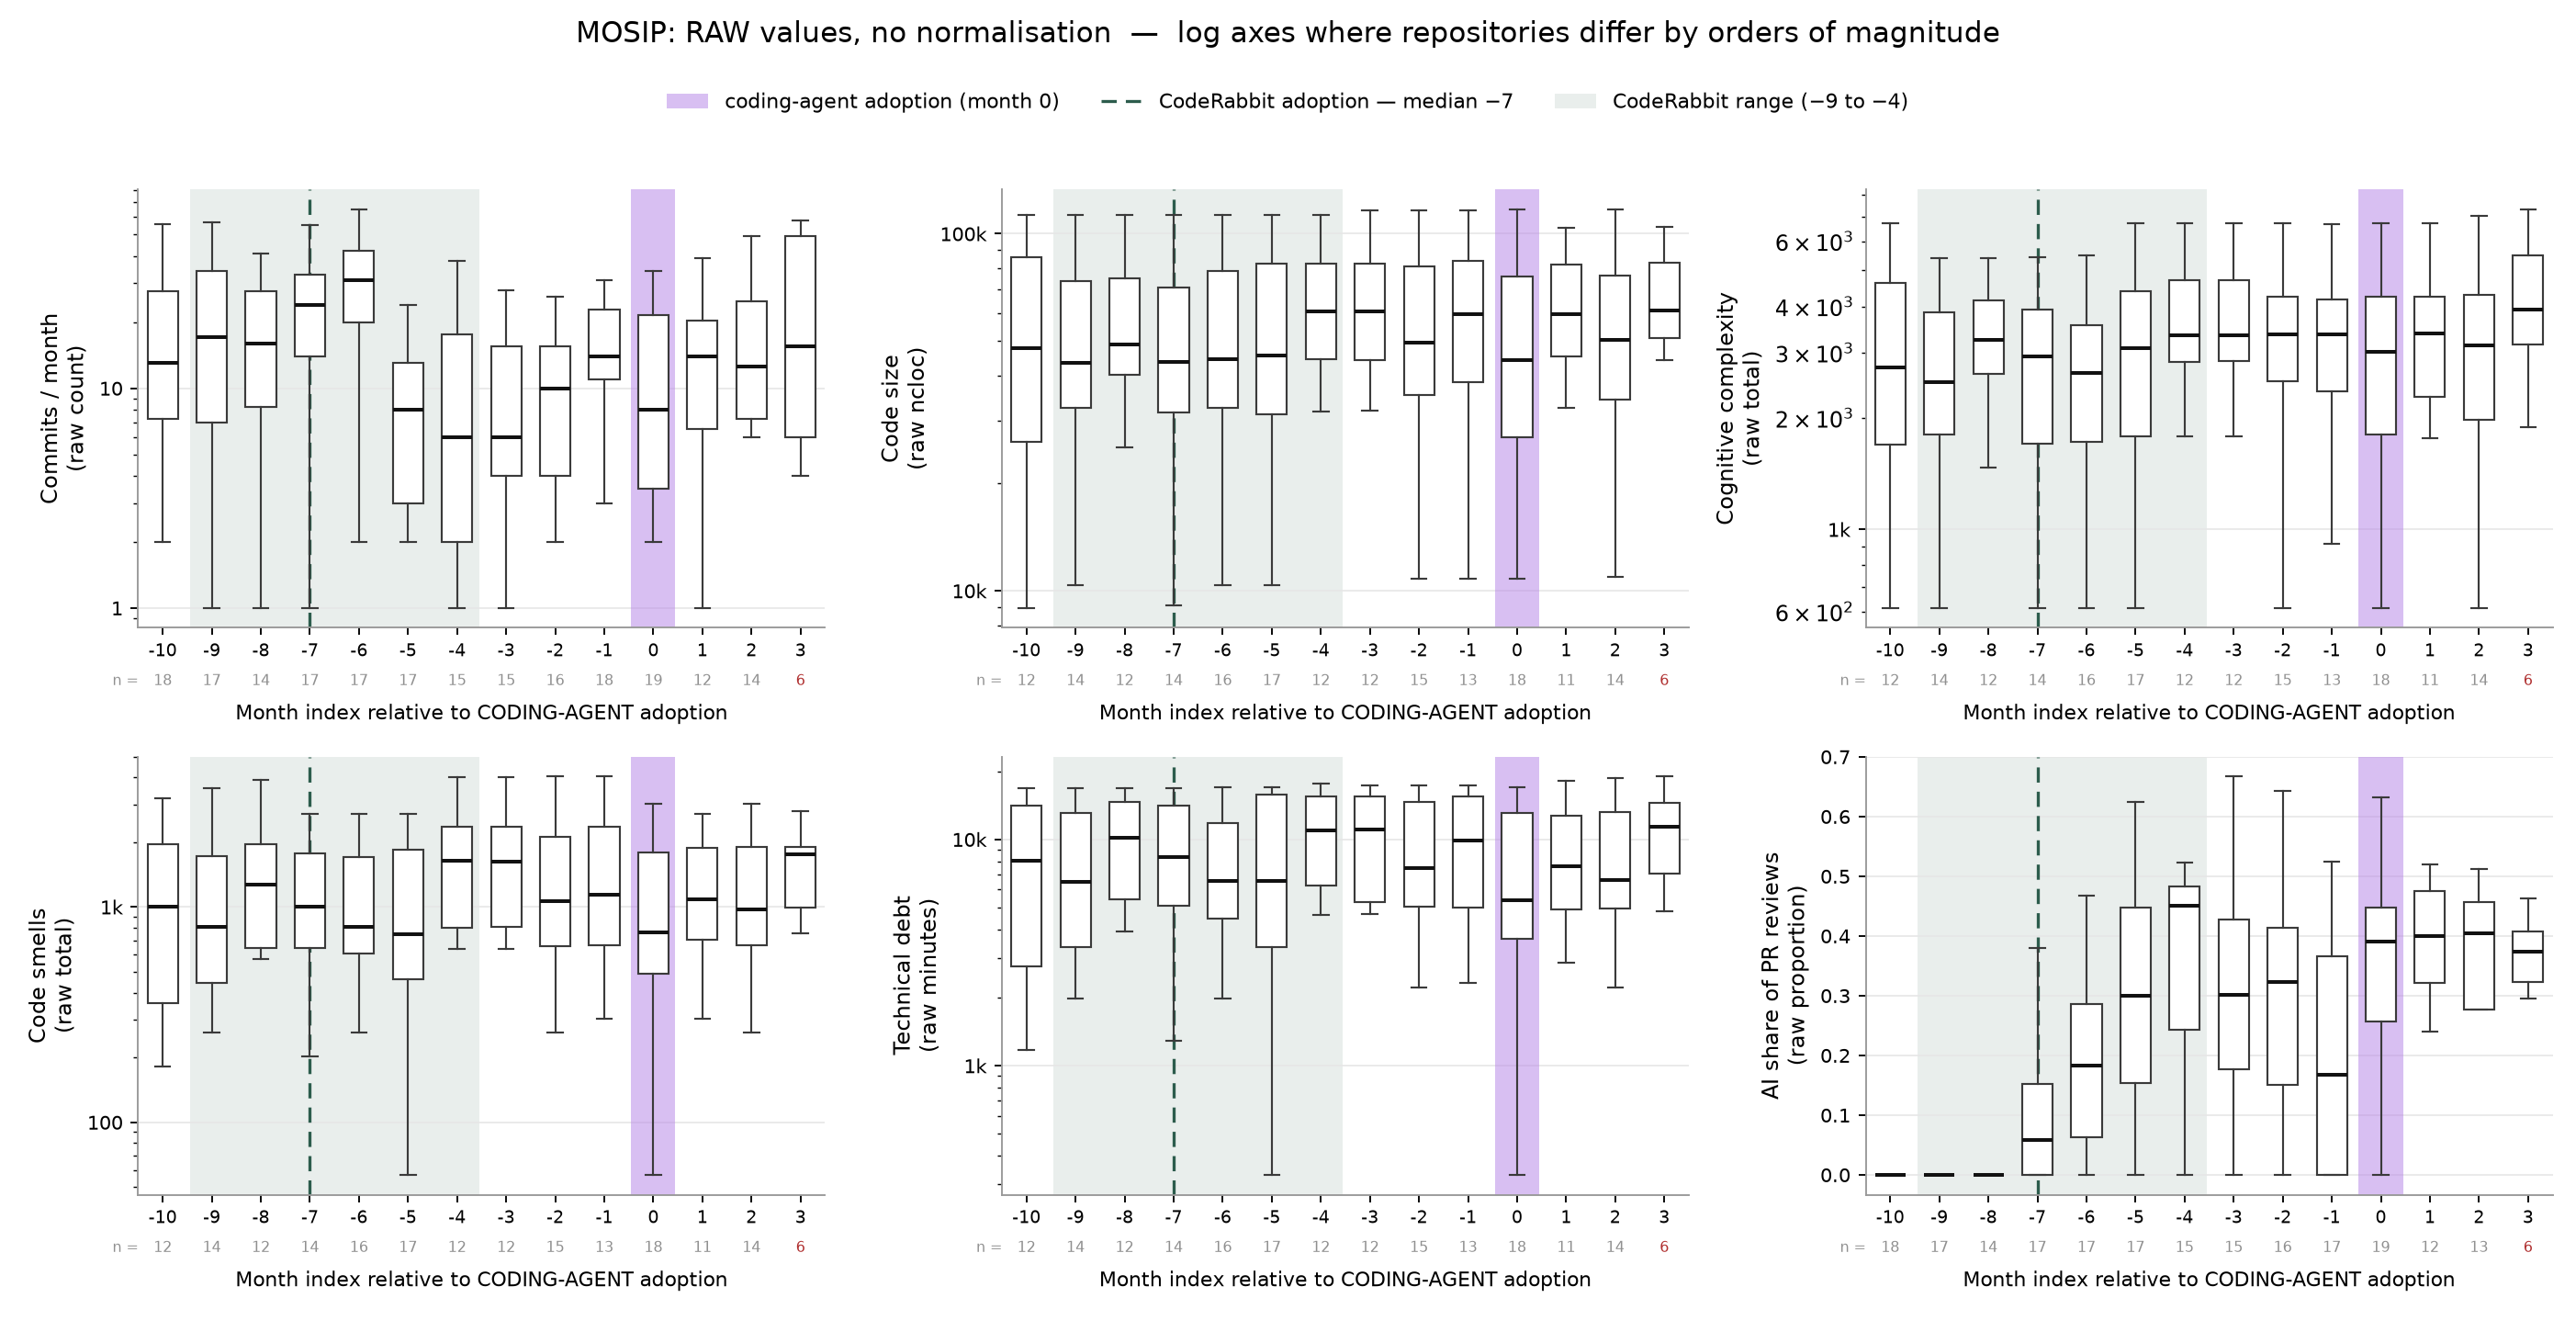
\includegraphics[width=\linewidth]{eventstudy.png}
  \caption{Event study on coding-agent adoption (purple band), all values raw.
  The earlier review-bot rollout appears as the dashed line at its median
  offset $\evt=-7$, with a band over its range. Axes are logarithmic where
  repositories differ by orders of magnitude. Box \emph{height} here is
  dominated by between-repository size rather than change over time; $n$
  beneath each box, red below 10.}
  \label{fig:eventstudy}
\end{figure}

\begin{figure}[htbp]
  \centering
  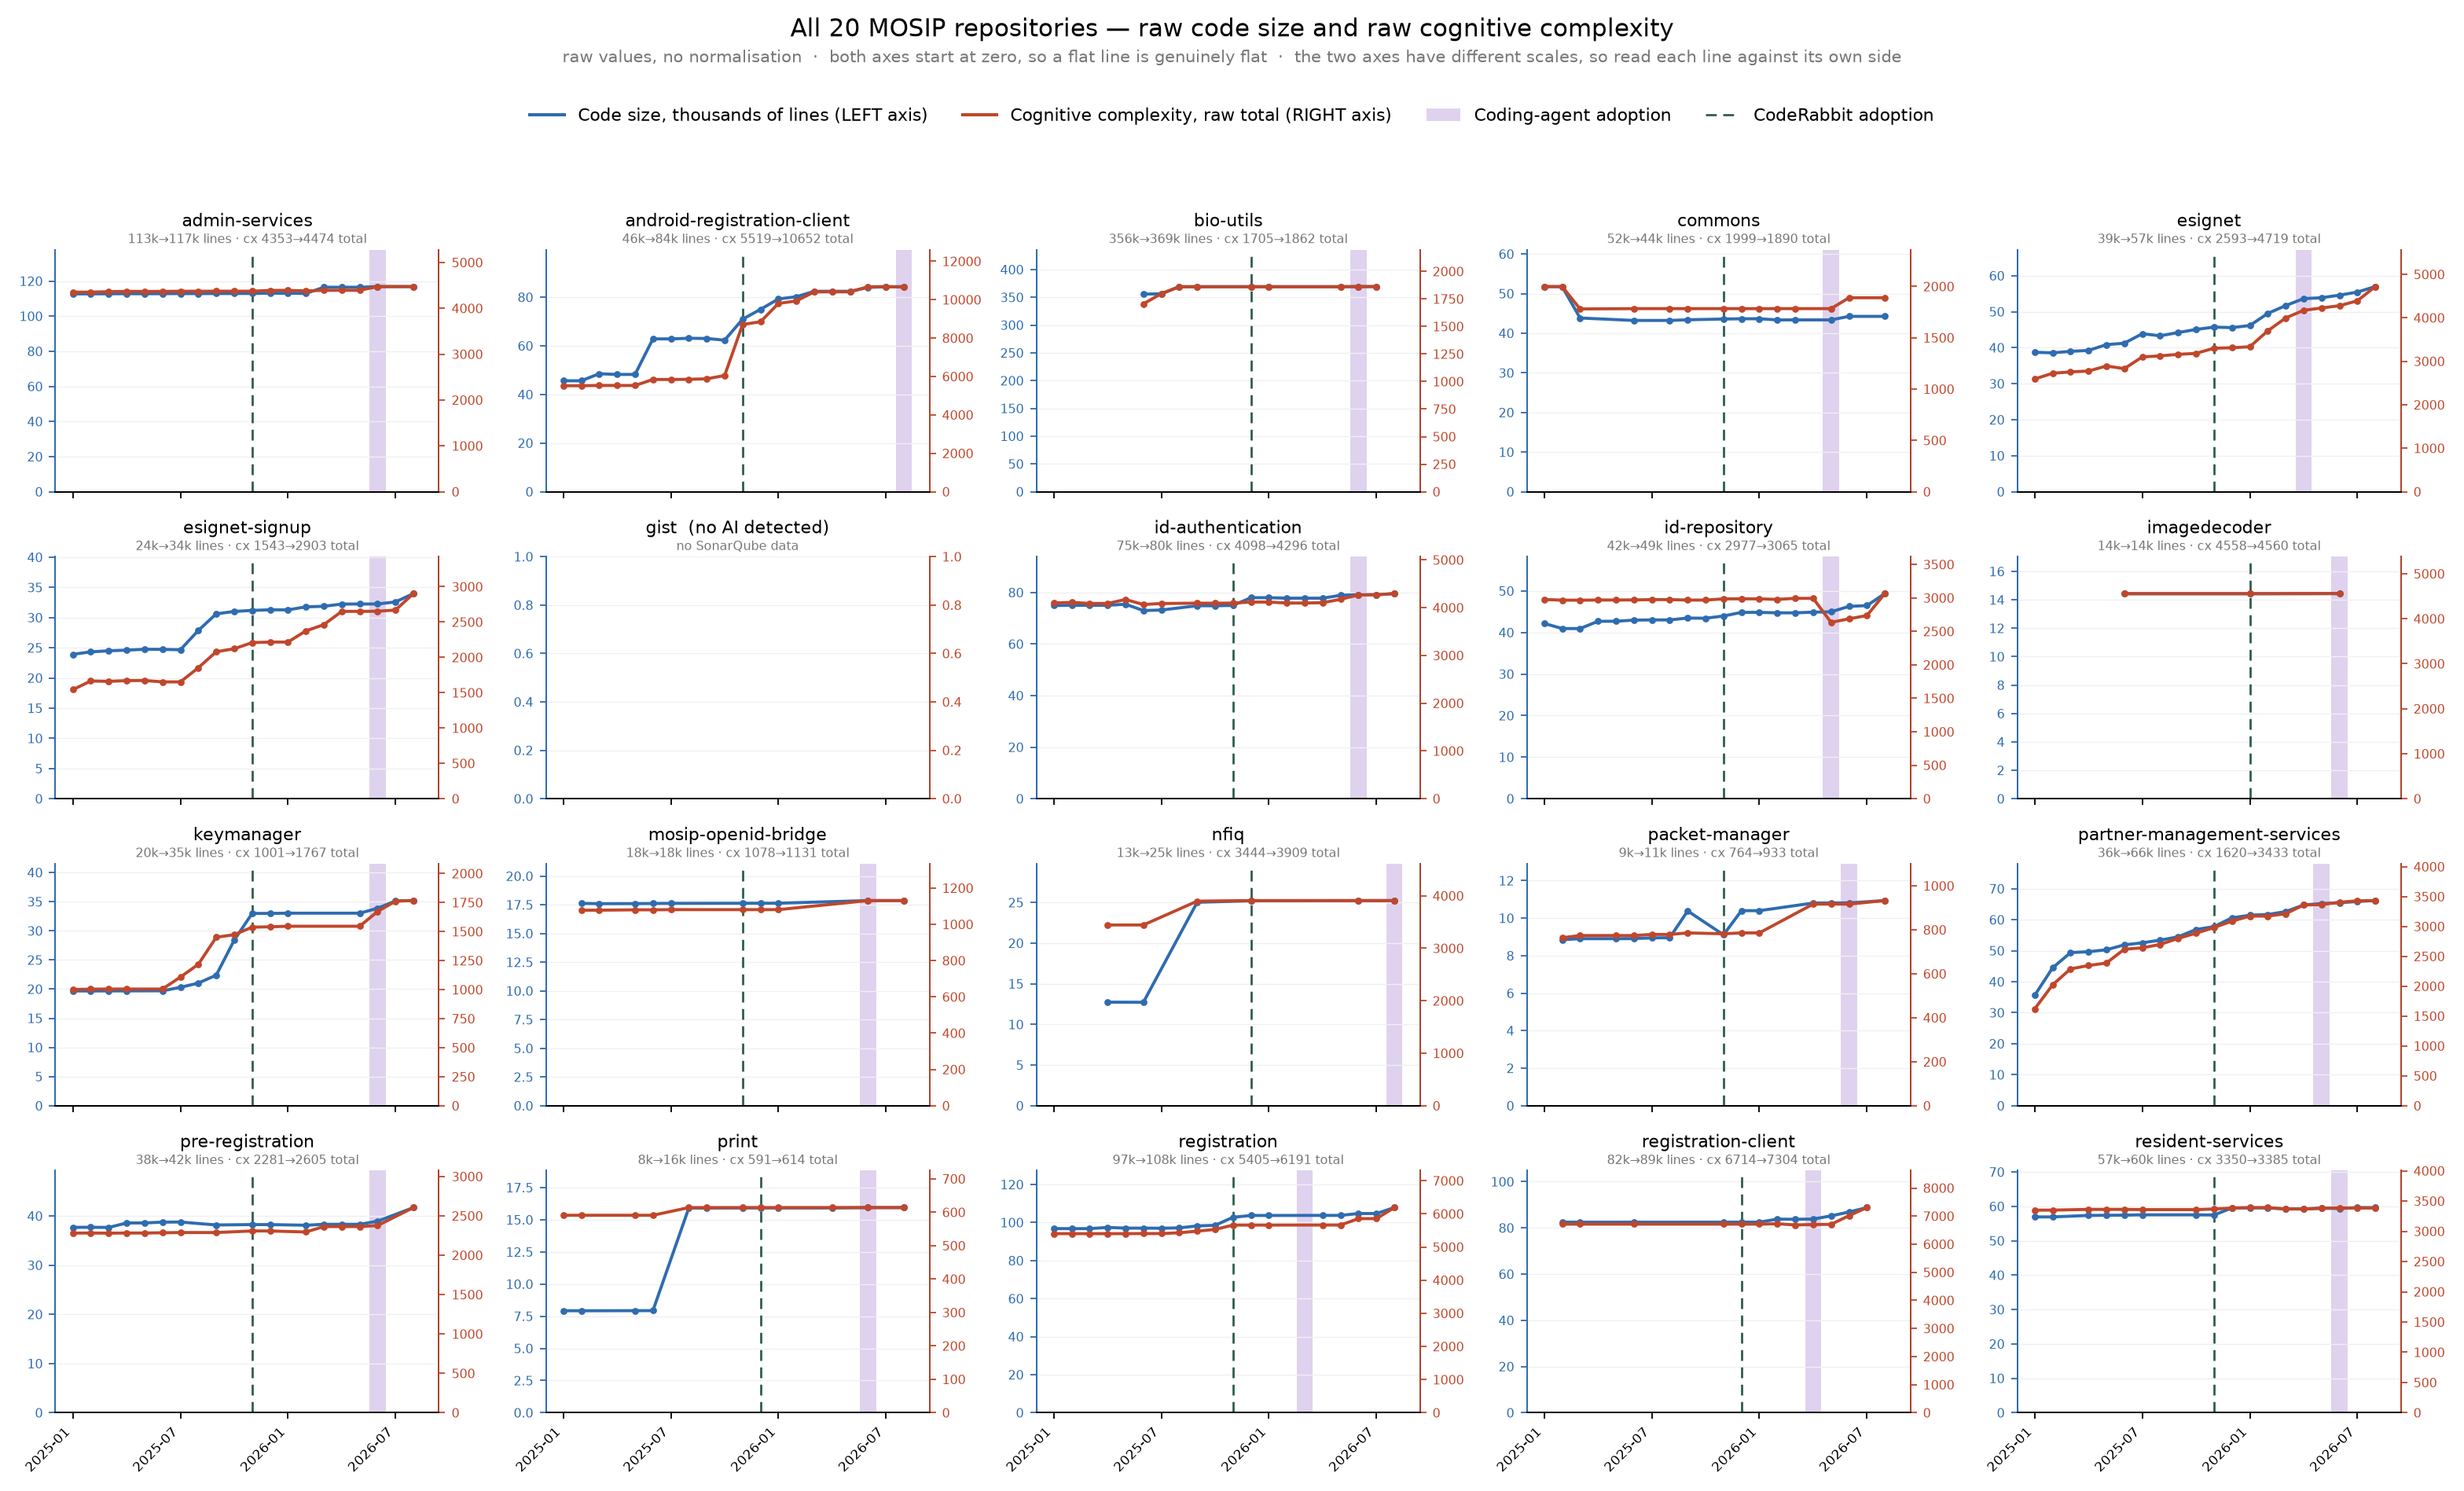
\includegraphics[width=\linewidth]{perrepo.png}
  \caption{Per-repository view, raw values, both axes anchored at zero. In most
  repositories the two lines track each other, the signature of complexity
  accumulating in step with code. The exceptions run both ways: \code{print}
  doubled in size (8k $\to$ 16k lines) with complexity almost flat
  (591 $\to$ 614), while \code{esignet-signup} grew 42\% in size
  (24k $\to$ 34k) but 88\% in complexity (1,543 $\to$ 2,903).}
  \label{fig:perrepo}
\end{figure}

Per repository, 17 of 19 grew in size (Figure~\ref{fig:perrepo}). Both
directions of the complexity relationship are present and should not be
averaged away.

%==============================================================================
\subsection{Code-review practices}
\label{sec:review}

RQ3 is evaluated against \textbf{review-bot} adoption, the relevant
intervention, with pre $=\evt\in[-6,-1]$ and post $=\evt\in[+1,+6]$. All counts
are raw.

\begin{table}[H]
\caption{Review practice, split at review-bot adoption.}
\label{tab:review}
\small
\begin{tabular}{@{}lNNNNN@{}}
\toprule
\textbf{Measure (raw)} & \textbf{pre} & \textbf{post} & \textbf{ratio} &
\textbf{p} & \textbf{n} \\
\midrule
\sigrow AI reviews / month & 0.0 & 6.0 & --- & \sig{.001} & 19 \\
Human reviews / month & 12.0 & 16.0 & \up{1.33} & .260 & 19 \\
\sigrow All reviews / month & 12.0 & 26.5 & \up{2.21} & \sig{.018} & 19 \\
\sigrow Human reviews / PR & \sig{1.43} & \sig{1.80} & \up{1.26} & \sig{.009} & 19 \\
\sigrow PRs opened / month & 12.5 & 8.0 & \dn{0.64} & \sig{.006} & 19 \\
\bottomrule
\end{tabular}
\end{table}

\begin{findingbox}{Finding 3}
The review bot was \textbf{additive, not substitutive}. Human review per pull
request \emph{rose} from 1.43 to 1.80 ($p=.009$), falling in only 6 of 19
repositories. Total review activity more than doubled. AI review accounts for
\textbf{26.1\%} of all 15,824 review submissions across the organisation.
\end{findingbox}

This is the clearest result in the study and the least threatened by the design
limitation in Section~\ref{sec:threats}, because the treatment indicator and
the outcome are the same class of event. The pre-adoption AI review share is
exactly zero in every repository in every month and rises to a plateau of
0.35--0.45 after adoption, which also validates the detection procedure end to
end.

\begin{cautionbox}{One competing explanation}
Pull-request volume fell 36\% over the same period ($12.5 \to 8.0$, $p=.006$).
Human reviews per PR could therefore rise because fewer, larger pull requests
each attract more attention rather than because reviewers became more engaged.
Distinguishing these requires conditioning on PR size, which we have not yet
done.
\end{cautionbox}

%==============================================================================
\esection{4 \textperiodcentered\ Threats to validity}{What this design cannot establish}
\label{sec:threats}

\begin{enumerate}
\item \textbf{Adoption is near-simultaneous, so event time is nearly collinear
with calendar time.} Fourteen of nineteen repositories adopted CodeRabbit in a
single month; $\mathrm{corr}(\evt,t)=0.997$ for the review wave and $0.980$ for
the coding wave. In the canonical two-way specification
\begin{equation}
  y_{it} = \alpha_i + \lambda_t
         + \sum_{k \neq -1} \beta_k \mathbf{1}[\evt_{it}=k] + \varepsilon_{it},
  \label{eq:twfe}
\end{equation}
common adoption $a_i = a$ implies
$\mathbf{1}[\evt_{it}=k] = \mathbf{1}[t=a+k]$, a deterministic function of
calendar time lying in the span of the time fixed effects, so $\beta_k$ is not
separately identified.

\item \textbf{Absolute counts confound quality with quantity.} Complexity and
smell totals necessarily rise in a growing codebase. Findings 1 and 2 report
real, separately measured quantities, but this study does not adjudicate
whether the quality increases exceed what growth alone implies.

\item \textbf{An organisation-wide slowdown.} Mean output fell from 24.4 to
14.5 commits per repository per month between 2025 and 2026, beginning months
before any coding agent. Every repository's pre/post boundary straddles it. We
therefore advance no velocity claim.

\item \textbf{Short post-adoption window.} Coding agents arrived mid-2026 and
the data ends 2026-08. By $\evt=+3$ only six repositories remain. Long-run
maintainability effects --- precisely what the literature
predicts~\cite{he2026speed} --- are not yet observable.

\item \textbf{Small treatment dose.} 147 commits are attributable to coding
agents across 326 repository-months.

\item \textbf{Unbalanced panel.} Repositories enter and leave columns; only
five appear at both $\evt=-10$ and $\evt=+3$. Because all tests are
within-repository this does not bias them, but raw cross-column comparisons in
the figures are unsafe.

\item \textbf{Single organisation.} MOSIP's engineering culture, review norms
and gitflow process are its own. Nothing here generalises without replication.
\end{enumerate}

\begin{goodbox}{What would establish causality}
A matched cohort of comparable non-adopting repositories observed over the same
calendar window. This is the only remedy for threat~1: because adoption is
near-simultaneous, additional MOSIP repositories would share the same timing
and the same shock, and would not help. The study's existing
\codep{matching\_simple.py} and \codep{analyze\_repos\_control.py} construct such
a cohort, and \codep{panel\_ai\_impact.csv} is already schema-compatible with
the difference-in-differences and panel-GMM notebooks.
\end{goodbox}

%==============================================================================
\esection{5 \textperiodcentered\ Summary}{Where this leaves the hypothesis}
\label{sec:conclusion}

Within one organisation, over a short post-adoption window, with a small
treatment dose: the code grew by 11\%, and its measured complexity and smell
counts grew by 2\% and 5\%. Technical debt, bugs and vulnerabilities did not
move; duplication improved. The direction is consistent with the population
literature~\cite{he2026speed}, but the magnitudes are substantially smaller
than the growth in code volume over the same interval, and this design cannot
separate either from a coincident organisational shock.

One contribution stands independently of the AI question. The distinction
between AI reviewers and AI writers is empirically consequential: these tools
arrived seven months apart, had different effects, and conflating them produces
attribution errors. The review-practice result in Section~\ref{sec:review} is
also the most robust finding here, because the outcome and the intervention are
the same class of event.

Next steps: construct a matched control cohort, which is the only remedy for
the identification problem in Section~\ref{sec:threats}; add a size-conditioned
analysis so Finding~2 can be read against what growth alone predicts; recompute
commit size as a true per-commit distribution, which also permits a
within-repository comparison of AI-authored against human-authored commits and
sidesteps the timing confound entirely; and re-run collection in six months,
when the post-adoption window will support the long-run question.

%==============================================================================
\section*{Data availability}

All figures and statistics are reproducible from the per-repository reports and
the pooled panel \codep{panel\_ai\_impact.csv} via the scripts in
\codep{\_tools/analysis/}. Tests use \codep{scipy.stats.wilcoxon}, two-sided, on
repository-level pairs.

\vspace{1em}
{\color{rule}\rule{\linewidth}{0.5pt}}
\vspace{0.5em}

{\ttfamily\scriptsize\color{muted}
Draft --- not for circulation. All values raw; no normalisation applied.\\
Descriptive before/after within a single organisation --- not a causal estimate.}

\bibliographystyle{plain}
\bibliography{references}

\end{document}
